\documentclass{amsart}
\usepackage{amssymb,amsmath,amsthm,mathrsfs,graphics,hyperref,ifthen,framed,cancel,fullpage,color,ytableau,tcolorbox,bm,tikz}
\usepackage[enableskew]{youngtab}
\raggedbottom
\parskip=10bp
\parindent=0bp
\raggedbottom

%%%%%%%%%%%%%%%%   Colors for TikZ and text  %%%%%%%%%%%%%%%%%

\definecolor{light}{gray}{.75}
\definecolor{med}{gray}{.5}
\definecolor{dark}{gray}{.25}
\newcommand{\Red}[1]{{\color{red}{#1}}}
\newcommand{\RED}[1]{{\color{red}{\boldmath\textbf{#1}\unboldmath}}}
\newcommand{\Blue}[1]{{\color{blue}{#1}}}
\newcommand{\BLUE}[1]{{\color{blue}{\boldmath\textbf{#1}\unboldmath}}}

% Hyperlinks
\hypersetup{colorlinks, citecolor=red, filecolor=black, linkcolor=blue, urlcolor=blue}
\newcommand{\hreftext}[2]{\href{#1}{\Blue{#2}}} % for text anchors
\newcommand{\hrefurl}[2]{\href{#1}{\Blue{\tt #2}}} % if you want to actually write out the URL in text

% Spacing and commands
\newcommand{\bigpad}{\rule[-14mm]{0mm}{30mm}}
\newcommand{\smallpad}{\rule[-1.5mm]{0mm}{5mm}}
\newcommand{\pad}{\rule[-3mm]{0mm}{8mm}}
\newcommand{\padup}{\rule{0mm}{5mm}}
\newcommand{\paddown}{\rule[-3mm]{0mm}{2mm}}
\newcommand{\blank}{\rule{1.25in}{0.25mm}}
\newcommand{\yell}[1]{\fbox{\rule[-1mm]{0mm}{4mm} \large\bf #1 }}
\newcommand{\indnt}{\phantom{.}\qquad}
\newcommand{\littleline}{\begin{center}\rule{4in}{0.5bp}\end{center}}

% macros for inserting figures
\newcommand{\includefigure}[3]{\begin{center}\resizebox{#1}{#2}{\includegraphics{#3}}\end{center}}
\newcommand{\includefigurewithinmath}[3]{\resizebox{#1}{#2}{\includegraphics{#3}}}
% E.g., to insert a standalone figure of width 3" and height 1.5", use
% \includefigure{3in}{1.5in}{foo.pdf}

% math operators
\DeclareMathOperator{\Comp}{Comp}
\DeclareMathOperator{\Fix}{Fix}
\DeclareMathOperator{\id}{id}
\DeclareMathOperator{\im}{im}
\DeclareMathOperator{\lcm}{lcm}
\DeclareMathOperator{\Par}{Par}
\DeclareMathOperator{\rank}{rank}
\DeclareMathOperator{\sh}{sh}
\DeclareMathOperator{\tr}{tr}
\DeclareMathOperator{\wt}{wt}

% theorem environments, automatically numbered
\newtheorem{theorem}{Theorem}[section]
\newtheorem{proposition}[theorem]{Proposition}
\newtheorem{lemma}[theorem]{Lemma}
\newtheorem{corollary}[theorem]{Corollary}
\theoremstyle{definition}
\newtheorem{definition}[theorem]{Definition}
\newtheorem{example}[theorem]{Example}
\newtheorem{remark}[theorem]{Remark}
\newtheorem{problem}[theorem]{Problem}

\newcommand{\skpr}{\emph{Sketch of proof: }}
\newcommand{\soln}{\textit{Solution:\ }}

% Generally useful macros
\newcommand{\excise}[1]{} % useful for commenting out large chunks
\newcommand{\0}{\emptyset}
\newcommand{\compn}{\models} % compositions
\newcommand{\dju}{\mathaccent\cdot\cup} % disjoint union
\newcommand{\dsum}{\displaystyle\sum}
\newcommand{\fallfac}[2]{{#1}^{\underline{#2}}} % falling factorial
\newcommand{\isom}{\cong} % isomorphism symbol
\newcommand{\partn}{\vdash} % partition symbol
\newcommand{\qqandqq}{\qquad\text{and}\qquad}
\newcommand{\qandq}{\quad\text{and}\quad}
\newcommand{\qand}{\quad\text{and}}
\newcommand{\qbin}[2]{{\begin{bmatrix}#1\\#2\end{bmatrix}_q}} % q-binomial coefficient
\newcommand{\risefac}[2]{{#1}^{\overline{#2}}} % rising factorial
\newcommand{\sd}{\triangle} % symmetric difference
\newcommand{\sm}{\setminus} % don't use a minus sign for this
\newcommand{\st}{\colon} % "such that"
\newcommand{\surj}{\twoheadrightarrow}
\newcommand{\x}{\times}

% blackboard bold fonts for sets of numbers
\newcommand{\Cc}{\mathbb{C}} % complex numbers
\newcommand{\Ff}{\mathbb{F}} % finite field
\newcommand{\Nn}{\mathbb{N}} % natural numbers
\newcommand{\Qq}{\mathbb{Q}}
\newcommand{\Rr}{\mathbb{R}}
\newcommand{\Zz}{\mathbb{Z}}

% miscellaneous
\newcommand{\TwoCases}[4]{\begin{cases}{#1}&\text{ #2}\\{#3}&\text{ #4}\end{cases}}
\newcommand{\ThreeCases}[6]{\begin{cases}{#1}&\text{ #2}\\{#3}&\text{ #4}\\{#5}&\text{ #6}\end{cases}}
\newcommand{\bridgehand}[4]{\spadesuit\ {\textsf{#1}}\ \ \heartsuit\ {\textsf{#2}}\ \ \diamondsuit\ {\textsf{#3}}\ \ \clubsuit\ {\textsf{#4}}}

% macros for automatic problem numbering --- students don't have to use these
\newcounter{probno}
\setcounter{probno}{0}
\newcounter{partno}
\setcounter{partno}{0}
%% versions that don't print the number of points
\newcommand{\prob}{
  \vskip10bp%
  \setcounter{partno}{0}%
  \addtocounter{probno}{1}%
  {\bf Problem~\#{\arabic{probno}}}\quad}

% No initial whitespace to make framing look nicer
\newcommand{\probns}{
  \setcounter{partno}{0}%
  \addtocounter{probno}{1}%
  {\bf Problem~\#{\arabic{probno}}}\quad}

\newcommand{\probpart}{%
  \addtocounter{partno}{1}%
  {\bf (\#\arabic{probno}\alph{partno})}\ \ }
\newcommand{\probcont}{%
  {\bf Problem~\#{\arabic{probno}}}~(\emph{continued})}
\newcommand{\probo}{
  \setcounter{partno}{0}%
  \addtocounter{probno}{1}%
  {\bf (\#\arabic{probno}}\ \ }

%% versions that do print the number of points
\newcommand{\Prob}[1]{
  \vskip10bp%
  \setcounter{partno}{0}%
  \addtocounter{probno}{1}%
  {\bf Problem~\#{\arabic{probno}}~[{#1}~pts]}\quad}

%no initial whitespace
\newcommand{\Probns}[1]{
  \setcounter{partno}{0}%
  \addtocounter{probno}{1}%
  {\bf Problem~\#{\arabic{probno}}~[{#1}~pts]}\quad}
\newcommand{\Probpart}[1]{%\rule{0in}{0in}\\ \phantom{xxx}
  \addtocounter{partno}{1}%
  {\bf (\#\arabic{probno}\alph{partno})~[{#1}~pts]}\ \ }

\newboolean{answers}
\newcommand{\Answer}[1]{\ifthenelse{\boolean{answers}}{{\bf Answer:}\ #1}{}\bigskip}

\begin{document}
\thispagestyle{empty}

\textbf{Math 724, Fall 2017\\
Homework \#6\\
Deadline: Wednesday, December 6, 5:00pm}

\textbf{Instructions:} Typeset your solutions in LaTeX.  Email your solutions to Jeremy (jlmartin@ku.edu) as a PDF file named with your last name and the problem set number (e.g., {\tt Germain6.pdf}).  Collaboration is encouraged, but each student must write up his or her solutions independently and acknowledge all collaborators.

\prob Bogart, Chapter 4, Supplementary Problem \#4.

\prob Bogart \#238 and \#239.  (Once you do \#238, problem \#239 should be easy.)

\prob The game of \textit{egdirb}, which does not really exist, uses a deck of 30 cards.  There are three suits: artichokes, ferrets, and pumpkins.  Each suit contains ten cards.  In one deal of egdirb, each of three players (Larry, Curly and Moe) receives a hand of 10 cards.  Use inclusion/exclusion to determine the probability that at least one player is dealt a void (i.e., zero cards) in at least one suit.

\prob Let $Y_n$ be the graph $K_n$ with one edge removed.  Find the chromatic polynomial of $Y_n$.

\prob \emph{Orienting} a graph means assigning a direction to each edge.  We can think of a directed edge as an arrow with a head and a tail.  There are two possible orientations for each edge (even loops --- you can think of the orientations as ``clockwise'' and ``counterclockwise''), so the total number of orientations of a graph with $e$ edges is $2^e$.

An orientation is \emph{acyclic} if there is no way to walk from any vertex back to itself by following one or more arrows.  The left-hand orientation is acyclic, but the right-hand orientation is not.

\begin{center}
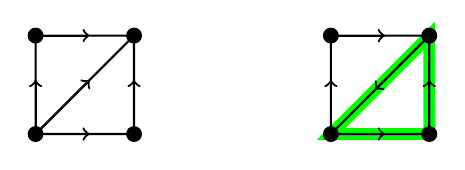
\begin{tikzpicture}[scale=1.25]
\newcommand{\ra}{0.075}
\draw[fill=black] (0,0) circle (\ra);
\draw[fill=black] (0,1) circle (\ra);
\draw[fill=black] (1,0) circle (\ra);
\draw[fill=black] (1,1) circle (\ra);
\draw[ thick] (0,0) -- (1,0) -- (1,1) -- (0,1) -- (0,0) -- (1,1);
\draw[ thick, ->] (0,0) -- (.55,0);
\draw[ thick, ->] (0,0) -- (.55,.55);
\draw[ thick, ->] (0,0) -- (0,.55);
\draw[ thick, ->] (1,0) -- (1,.55);
\draw[ thick, ->] (0,1) -- (.55,1);
\begin{scope}[shift={(3,0)}]
\draw[line width=1.5mm,green] (0,0) -- (1,0) -- (1,1) -- cycle;
\draw[fill=black] (0,0) circle (\ra);
\draw[fill=black] (0,1) circle (\ra);
\draw[fill=black] (1,0) circle (\ra);
\draw[fill=black] (1,1) circle (\ra);
\draw[ thick] (0,0) -- (1,0) -- (1,1) -- (0,1) -- (0,0) -- (1,1);
\draw[ thick, ->] (0,0) -- (.55,0);
\draw[ thick, ->] (1,1) -- (.45,.45);
\draw[ thick, ->] (0,0) -- (0,.55);
\draw[ thick, ->] (1,0) -- (1,.55);
\draw[ thick, ->] (0,1) -- (.55,1);
\end{scope}
\end{tikzpicture}
\end{center}


Let $A(G)$ denote the set of acyclic orientations of $G$, and let $\alpha(G)=|A(G)|$.

(5a) What is $\alpha(G)$ if $G$ is a forest?  What is $\alpha(K_n)$?  What is $\alpha(C_n)$?  (Here $K_n$ is the complete graph with $n$ vertices, and
$C_n$ is the cycle graph of length~$n$.)
To get at these counting problems (particularly for $K_n$), observe the following.  Any labeling of the vertices of $G$ by distinct real numbers (say $1,\dots,n$, where $n$ is the number of vertices) gives rise to an orientation by pointing every edge toward its larger endpoint.  This orientation is always acyclic (why?)  Do different labelings always induce different orientations?  Does every orientation of $G$ arise in this way?

(5b) Show that $\alpha(G)=\alpha(G-e)+\alpha(G/e)$ for any edge $e$.

Hint: Consider the map $\pi:A(G)\to A(G-e)$ given by forgetting the orientation of $e$.  First, show that $\pi$ is onto.  Second, figure out which acyclic orientations of $A(G-e)$ arise from one acyclic orientation of $G$ and which from two.  This should give you a combinatorial interpretation for the ``overcount'' $\alpha(G)-\alpha(G-e)$.  Use a bijection to show that this overcount is exactly $\alpha(G/e)$.

(5c) Find a formula for $\alpha(G)$ in terms of the chromatic polynomial $\chi_G(k)$.
(The answer should knock your socks off!)

(5d) Label the vertices of $G$ by $1,\dots,n$.  For each edge $ij\in E(G)$, define a hyperplane $H_{ij}\subset\Rr^n$ by
\[H_{ij} = \{(x_1,x_2\dots,x_n)\in\Rr^n \st x_i=x_j\}\]
and define
\[\mathcal{A}_G = \bigcup_{ij\in E} H_{ij}.\]
Thus $\mathcal{A}_G$ is a subset of $\Rr^n$; it is called a \emph{graphical hyperplane arrangement}.  Show that there is a bijection between $A(G)$ and the connected components of $\Rr^n\sm\mathcal{A}_G$.

\prob
Let $V=[n]$ and let $G$ be a graph with vertex set $V$.
The \emph{chromatic symmetric function} (CSF) of $G$ is the formal power series
defined by
\[X(G) = \sum_f \prod_{i=1}^n x_{f(i)}\]
where the sum ranges over all proper colorings $f$.  Note that this is a power series in infinitely many variables.  An equivalent definition is
\[X(G) = \sum_f \prod_{j=1}^\infty x_j^{c_j(f)}\]
where $c_j(f)$ is the number of vertices that are assigned color~$j$ by the coloring~$f$.  So $X(G)$ keeps track not only of the number of proper colorings, but also of how many proper colorings use each possible distribution of colors.  The term ``symmetric'' means that it is invariant under permutations of the variables (because, e.g., the number of proper colorings of $G$ with three blue, one red and two pink vertices equals the number with three green, one pink and two sepia).

There is a convenient way of describing $X(G)$ that does not require writing out the complete power series.  Given a partition $\lambda\partn n$, let $c_\lambda(G)$ be the number of proper colorings with $\lambda_1$ parts of color 1, $\lambda_2$ parts of color 2, etc.  Then $c_\lambda(G)$ is the coefficient in $X(G)$ of any monomial of the form $x_{i_1}^{\lambda_1}x_{i_2}^{\lambda_2}\cdots$, where $i_1,i_2,\dots$ are all distinct.  (The number of proper colorings with three fuchsia, one aquamarine, and two silver vertices is $c_{321}$.)  Therefore $X(G)$ is specified exactly by the list of numbers $c_\lambda(G)$ for all $\lambda\partn n$.

For example, let $G$ be the unique tree with three vertices.  There are
6 ways to color one vertex red, one vertex blue and one vertex green (since every such coloring is proper, and there are $3!=6$ such colorings), so $c_{111}=6$.
There is 1 way to color one vertex red and two vertices blue (the red vertex must be the one in the center).  It is impossible to color all three vertices magenta.  So $X(G)$ is completely specified by the values
\[c_{111}(G)=6, \quad c_{21}(G)=1,\quad c_{3}(G)=0.\]

%\begin{center}
%\begin{tikzpicture}[scale=1.25]
%\newcommand{\ra}{0.075}
%\draw[fill=black] (0,1) circle (\ra);
%\draw[fill=black] (1,0) circle (\ra);
%\draw[fill=black] (2,1) circle (\ra);
%\draw[thick] (0,1) -- (1,0) -- (2,1);
%\node at (0,0) {$P_3$};
%
%\foreach \x in {4,5,6} { \draw[fill=black] (\x,1) circle (\ra); \draw[thick] (\x,1) -- (5,0); }
%\draw[fill=black] (5,0) circle (\ra);
%\node at (4,0) {(b)};
%
%\draw[fill=black] (8,1) circle (\ra);
%\draw[fill=black] (9,0) circle (\ra);
%\draw[fill=black] (10,1) circle (\ra);
%\draw[fill=black] (11,0) circle (\ra);
%\draw[thick] (8,1) -- (9,0) -- (10,1) -- (11,0);
%\node at (8,0) {(c)};
%\end{tikzpicture}
%\end{center}

(6a) What is $X(G)$ if $G$ has no edges?  What is $X(K_n)$?  (Here you can actually describe the power series.)

(6b) Explain how to derive the number of proper $k$-colorings from $X(G)$, for any positive integer $k$.  (Be careful: there is not (to my knowledge) an easy algebraic specialization of $X(G)$ that yields the polynomial $\chi_G(k)$ --- but for any \emph{number} $k$, it is possible to obtain the \emph{number} $\chi_G(k)$ from $X(G)$.  Therefore, all information about $G$ that can be obtained from $\chi_G$ can in principle be obtained from $X(G)$.

(6c) There are (up to isomorphism) two trees on four vertices, the path $P_4$ and the star $K_{3,1}$.  Show that they do \emph{not} have the same CSF, even though they have the same chromatic polynomial.

(6d) Do the same for the three trees on five vertices.  (It is unknown whether two nonisomorphic trees can have the same CSF.  This is an open problem that has caused Jeremy many sleepless nights.)

\end{document}